\documentclass{article}
\usepackage[utf8]{inputenc}
\usepackage{graphicx}

\title{TUGAS BESAR BASIS DATA II\\
Aplikasi Barbershop}
\author{Helmi Azhar 1184013\\
D4 Teknik Informatika 2C}
\date{Desember 2019}

\begin{document}

\maketitle
\section{Oracle Apex}

\begin{enumerate}
\usepackage{Oracle Apex merupakan suatu aplikasi atau tools  untuk memudahkan apa yang kita butuhkan. Sesuai namanya, oracle express bila dipelajari lebih dalam banyak memberi kemudahan dalam melayanani kebutuhan user contohnya dalam pembuatan aplikasi sederhana,belajar function dan lain-lain. Oracle apex juga dapat mengembangkan aplikasi web desktop dan seluler, memvisualisasikan dan memelihara data basis data, dan meningkatkan keterampilan sql dan kemampuan basis data}
\end{enumerate}

\section{Langkah-langkah}
\begin{itemize}
        \item Sign in pada Oracle Application Express
        \begin{center}
        \centering
        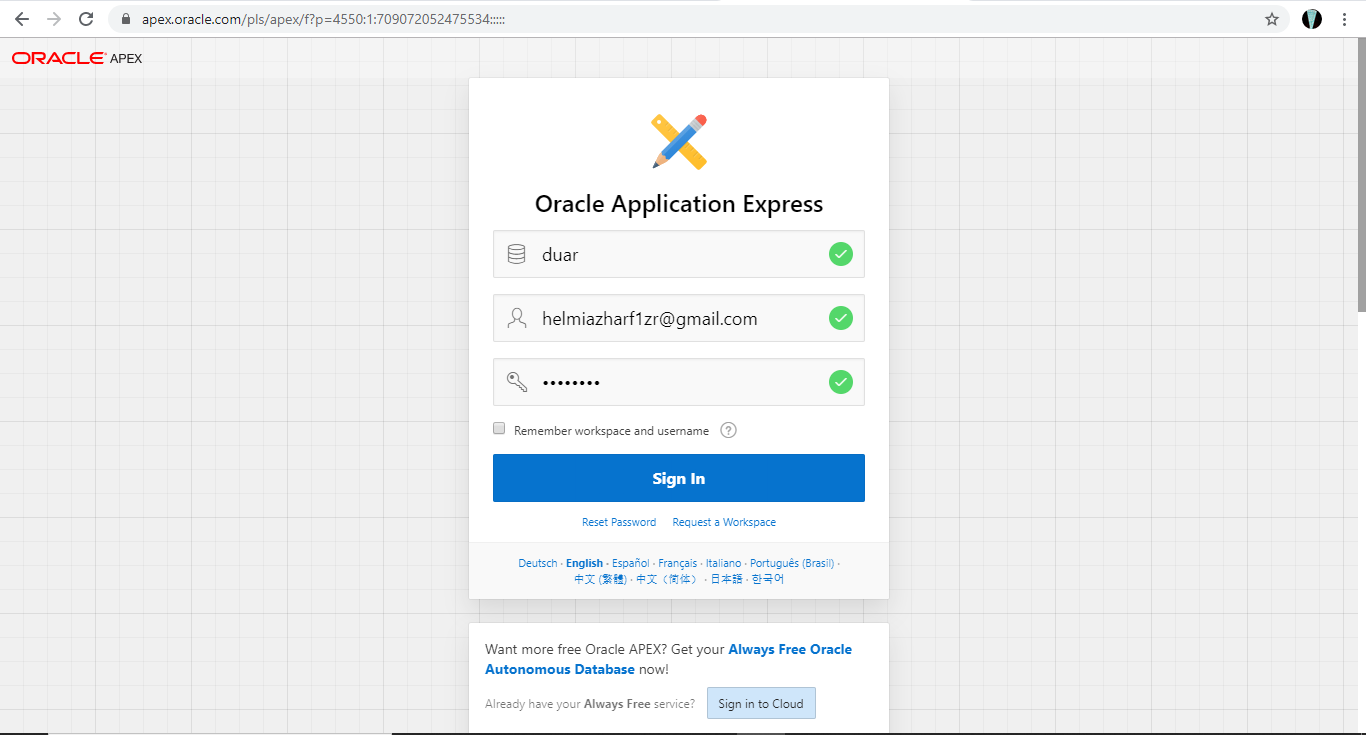
\includegraphics[scale=0.3]{gambar/1.PNG}
    \end{center}
    
        \item Setelah masuk klik SQL Workshop dibagian atas lalu pilih SQL Commands untuk membuat tabel barber dan pelanggan
        \begin{center}
        \centering
        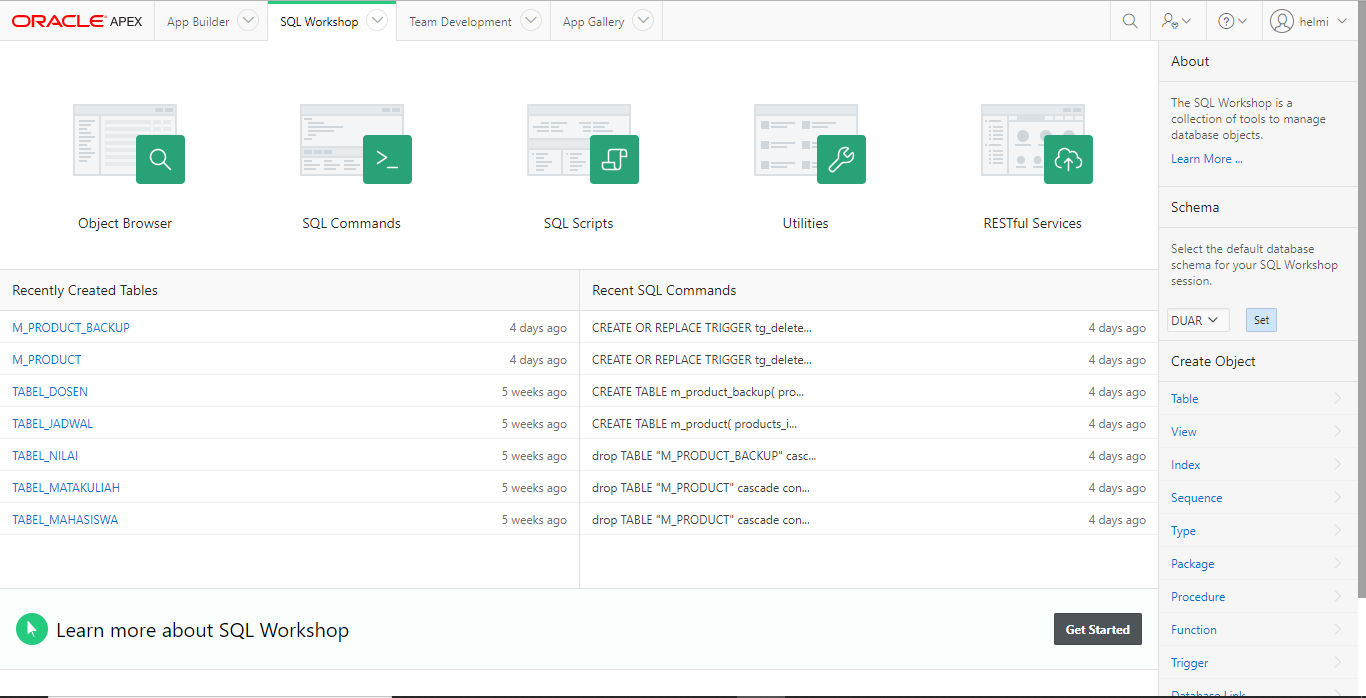
\includegraphics[scale=0.3]{gambar/2.PNG}
    \end{center}
    
        \item buat tabel barber setelah itu run 
        \begin{center}
        \centering
        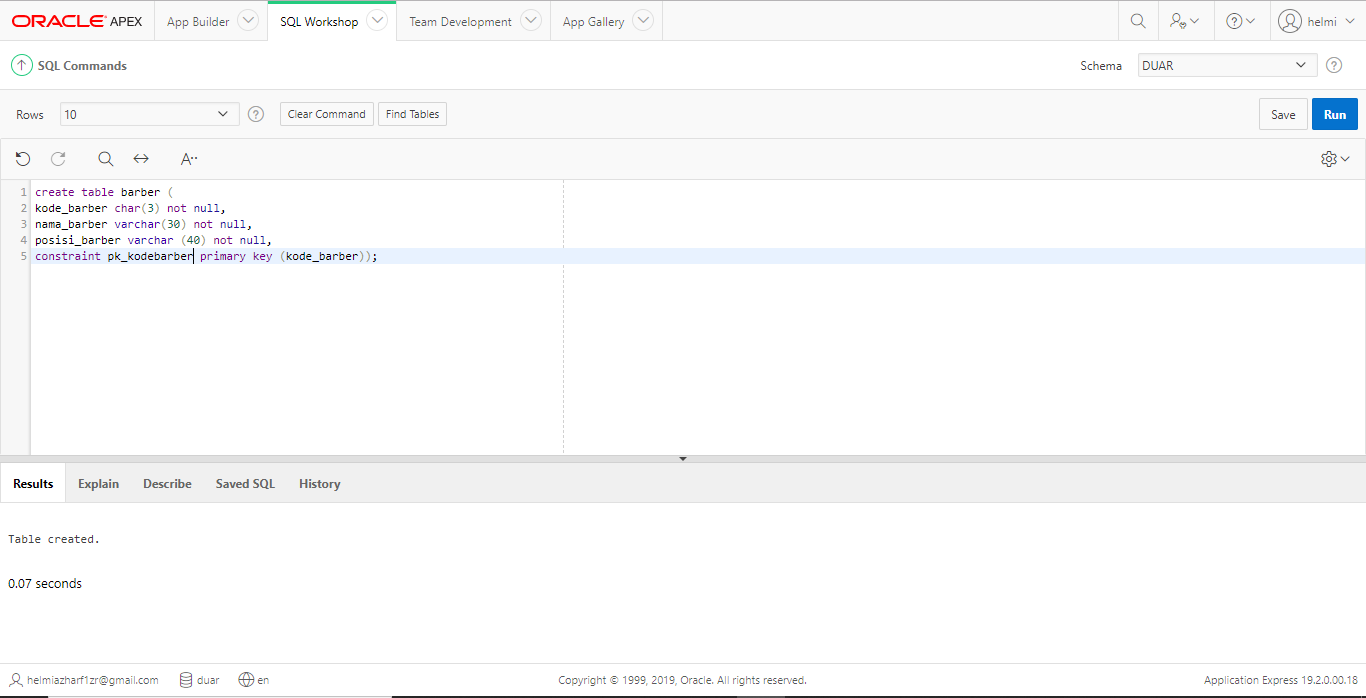
\includegraphics[scale=0.3]{gambar/3.PNG}
    \end{center}
    
        \item buat tabel pelanggan setelah itu run 
        \begin{center}
        \centering
        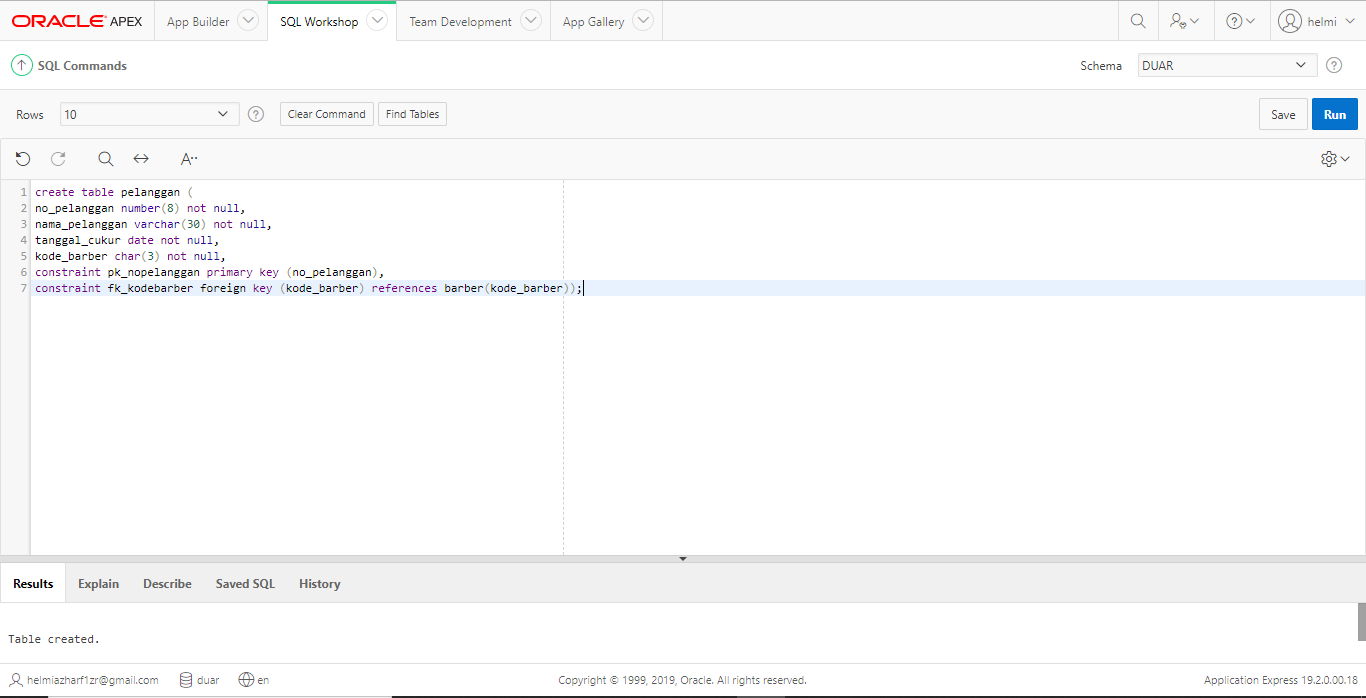
\includegraphics[scale=0.3]{gambar/4.PNG}
    \end{center}
        
        \item buat tabel history pelanggan setelah itu run 
        \begin{center}
        \centering
        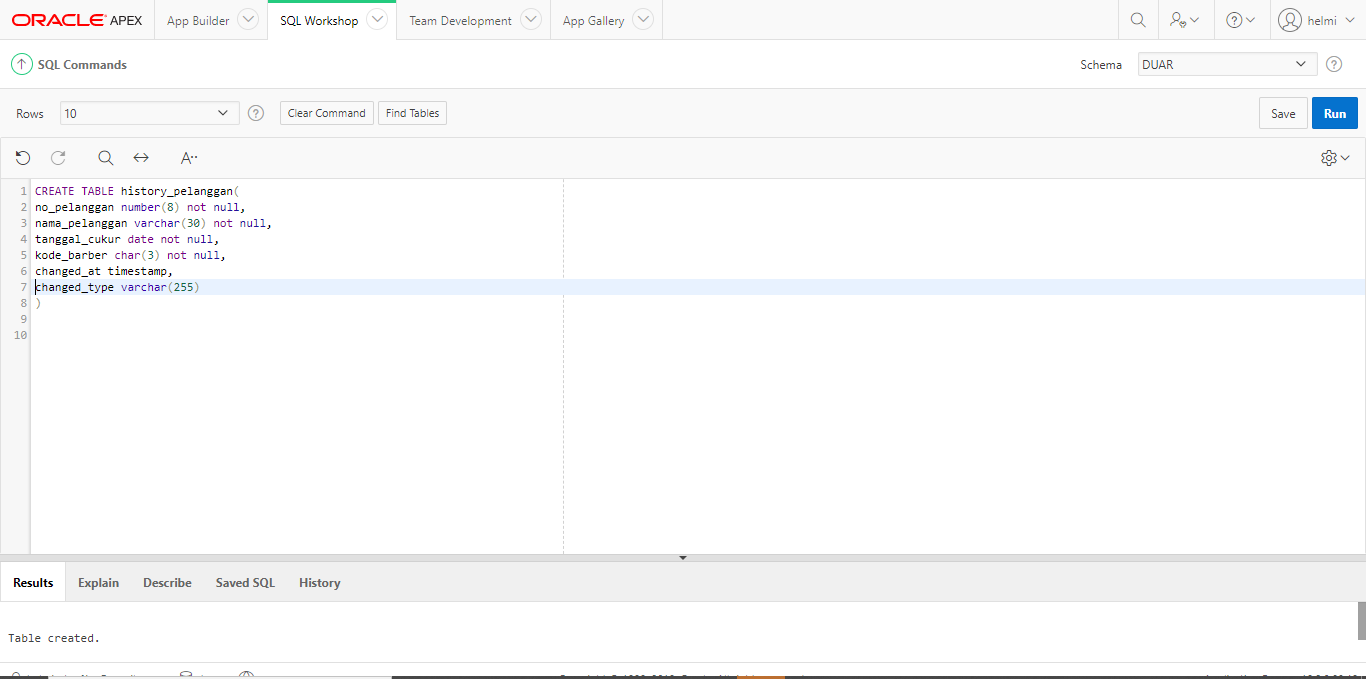
\includegraphics[scale=0.3]{gambar/6.PNG}
    \end{center}
    
        \item buat triger delete untuk pelanggan, lalu run
        \begin{center}
            \centering
            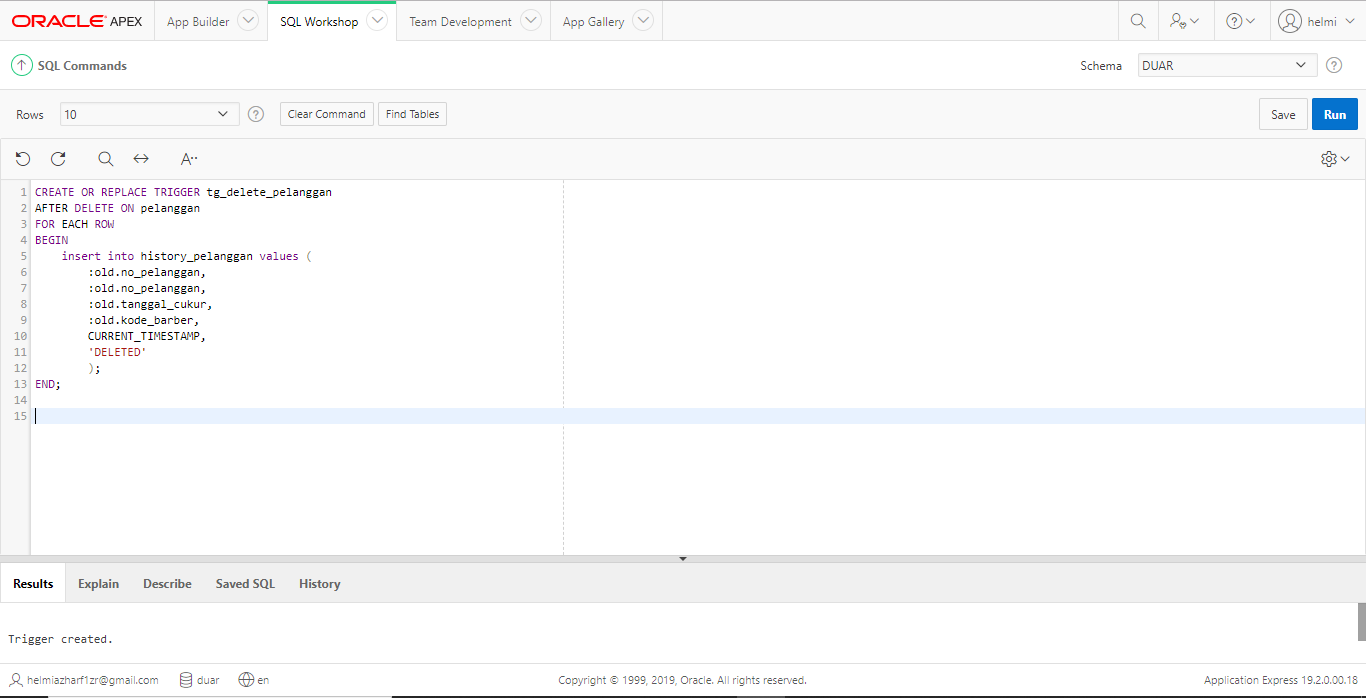
\includegraphics[scale=0.3]{gambar/7.PNG}
        \end{center}
        
        \item buat triger update untuk pelanggan,lalu run
        \begin{center}
            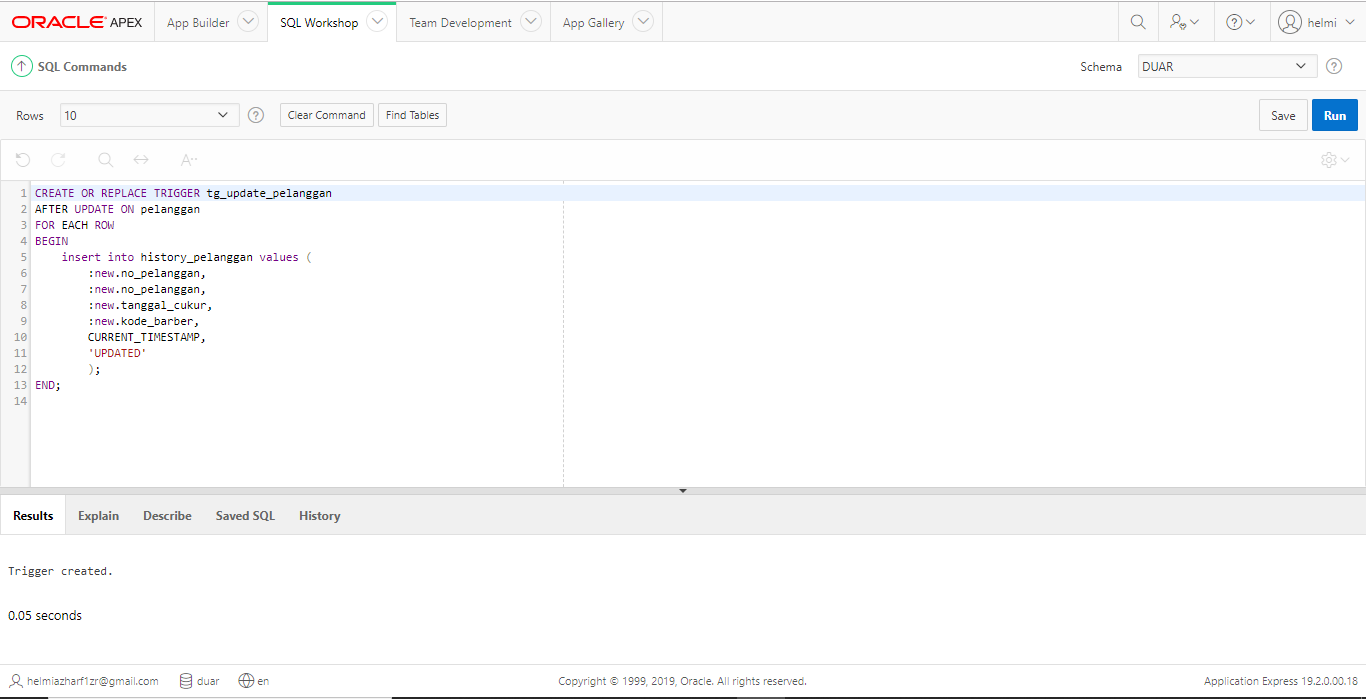
\includegraphics[scale=0.3]{gambar/9.PNG}
        \end{center}
        
        \item buat view untuk melihat siapa saja yang menggunakan jasa barbernya
        \begin{center}
            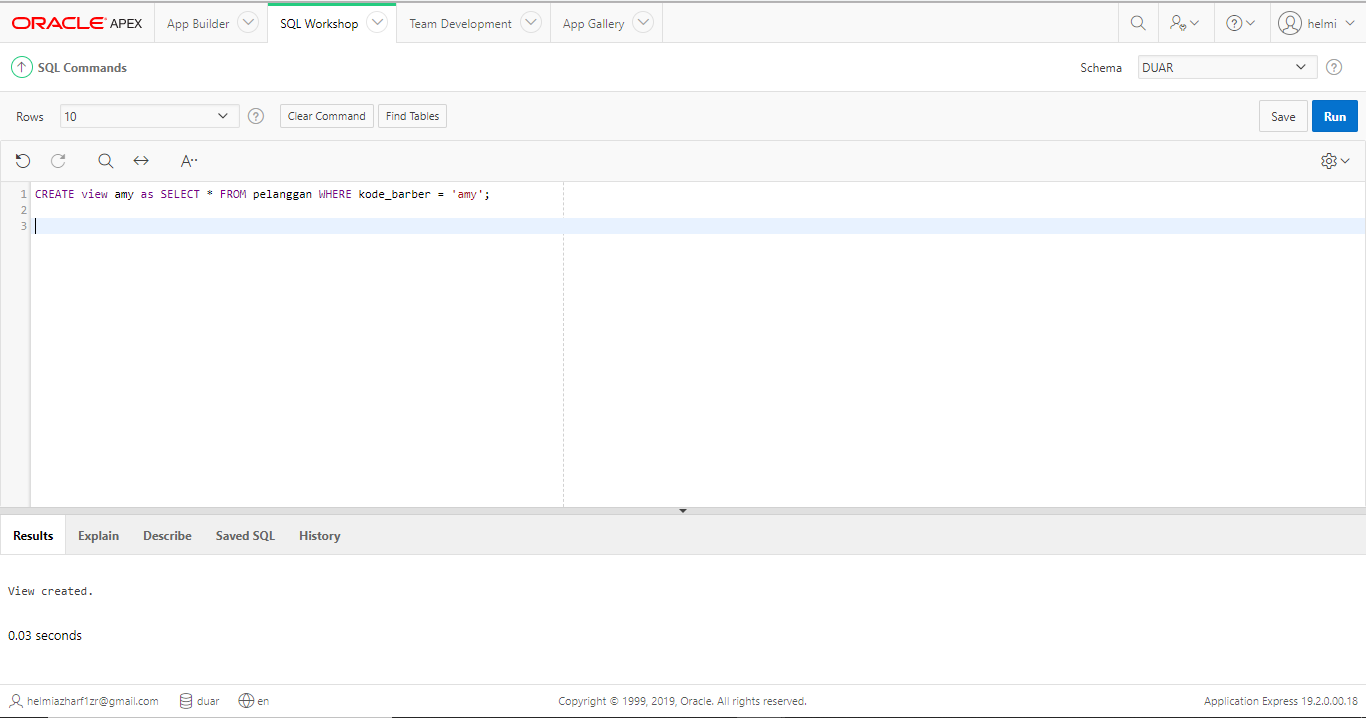
\includegraphics[scale=0.3]{gambar/view.PNG}
        \end{center}
        
        \item buat triger insert untuk pelanggan,setelah dirun buka pilihan pada app builder lalu pilih create
        \begin{center}
            \centering
            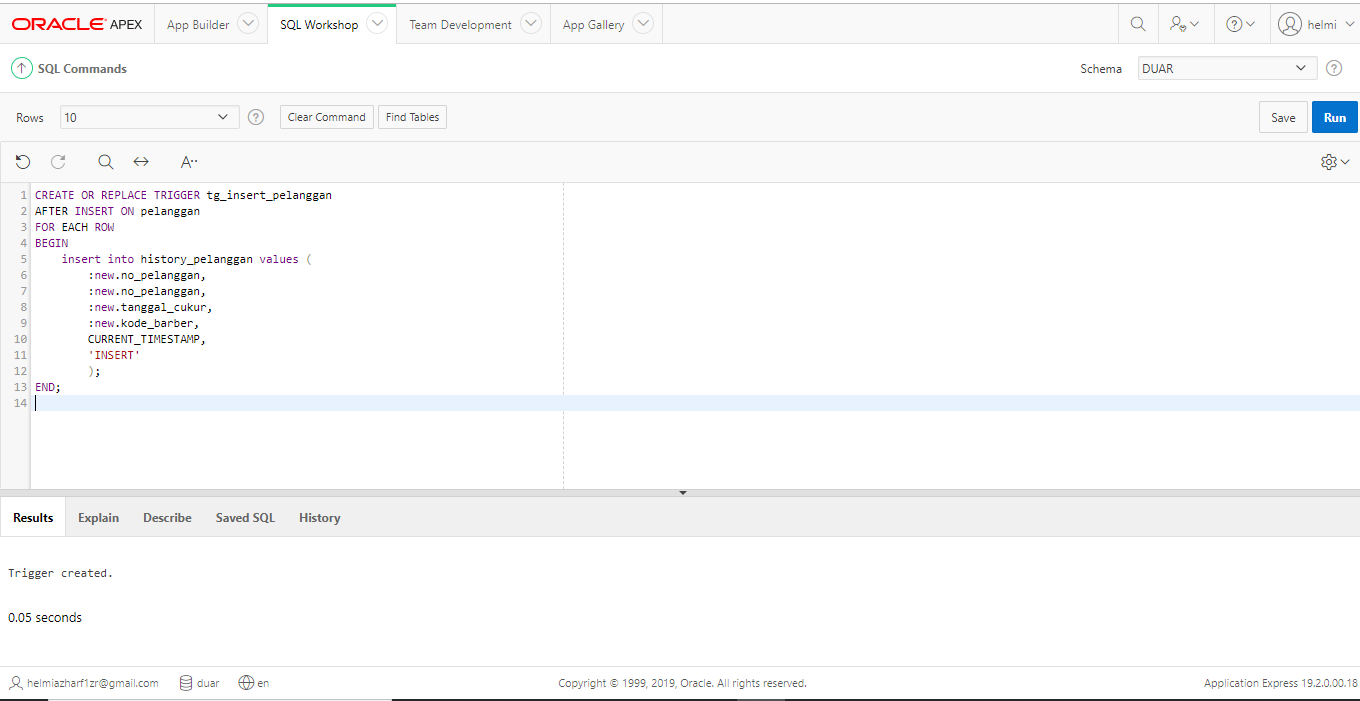
\includegraphics[scale=0.3]{gambar/8.PNG}
        \end{center}
        
        \item pilih New Application 
        \begin{center}
        \centering
        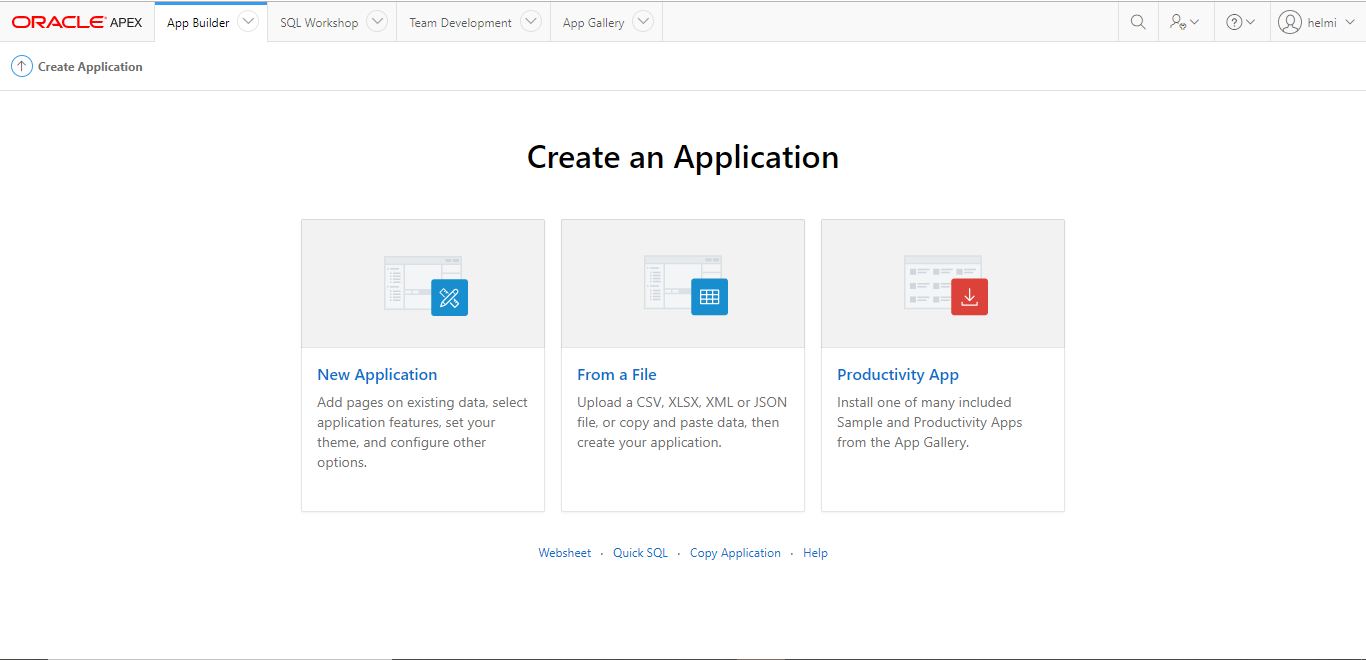
\includegraphics[scale=0.3]{gambar/5.PNG}
    \end{center}

        \item Isi nama aplikasi lalu add page
        \begin{center}
            \centering
            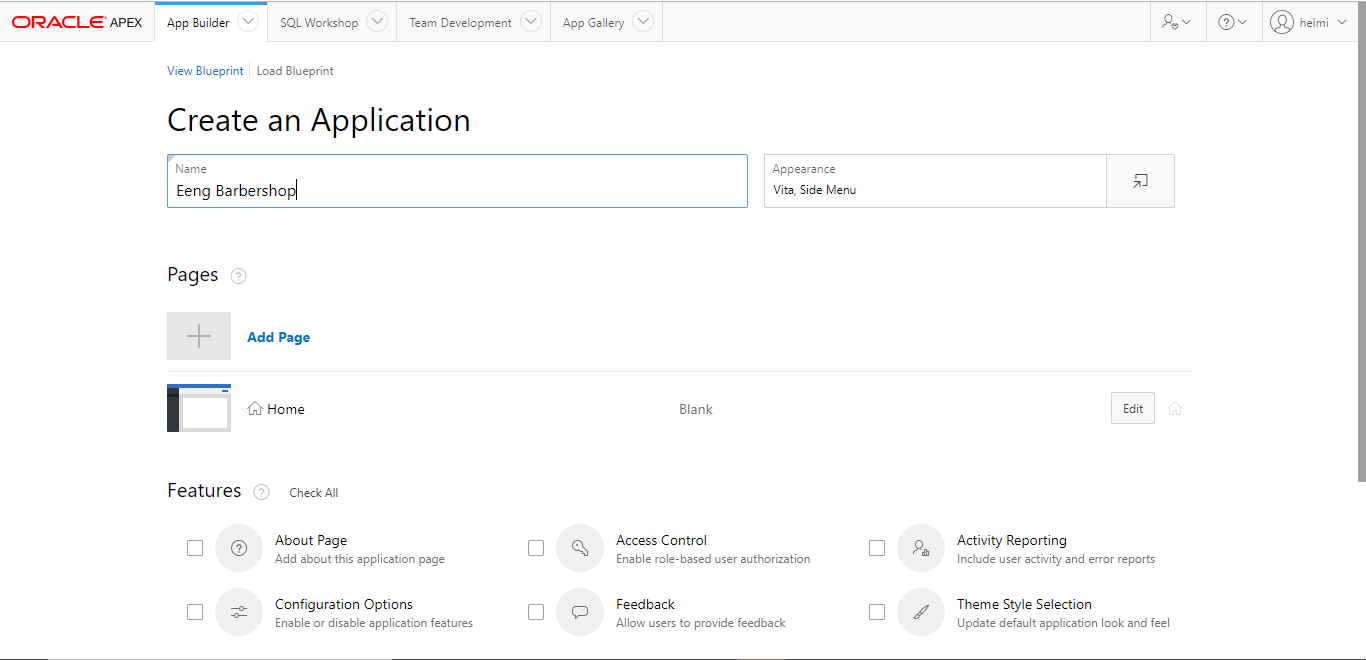
\includegraphics[scale=0.3]{gambar/10.PNG}
        \end{center}

        \item pilih interactive report untuk menampilkan data pelanggan yang akan dicukur dan pilih tabel pelanggan lalu page add page 
        \begin{center}
            \centering
            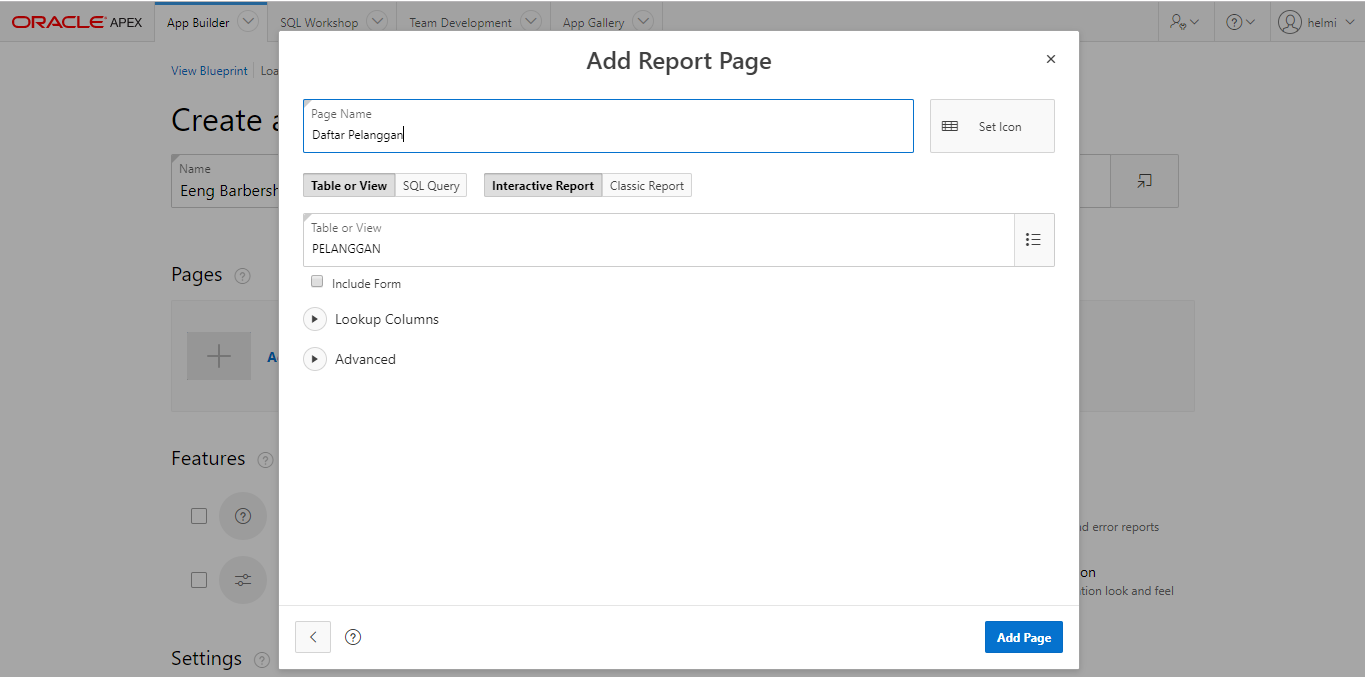
\includegraphics[scale=0.3]{gambar/11.PNG}
        \end{center}
        
        \item pilih interactive report untuk menampilkan data pelanggan yang akan dicukur oleh helmi dan pilih view amy lalu page add page 
        \begin{center}
            \centering
            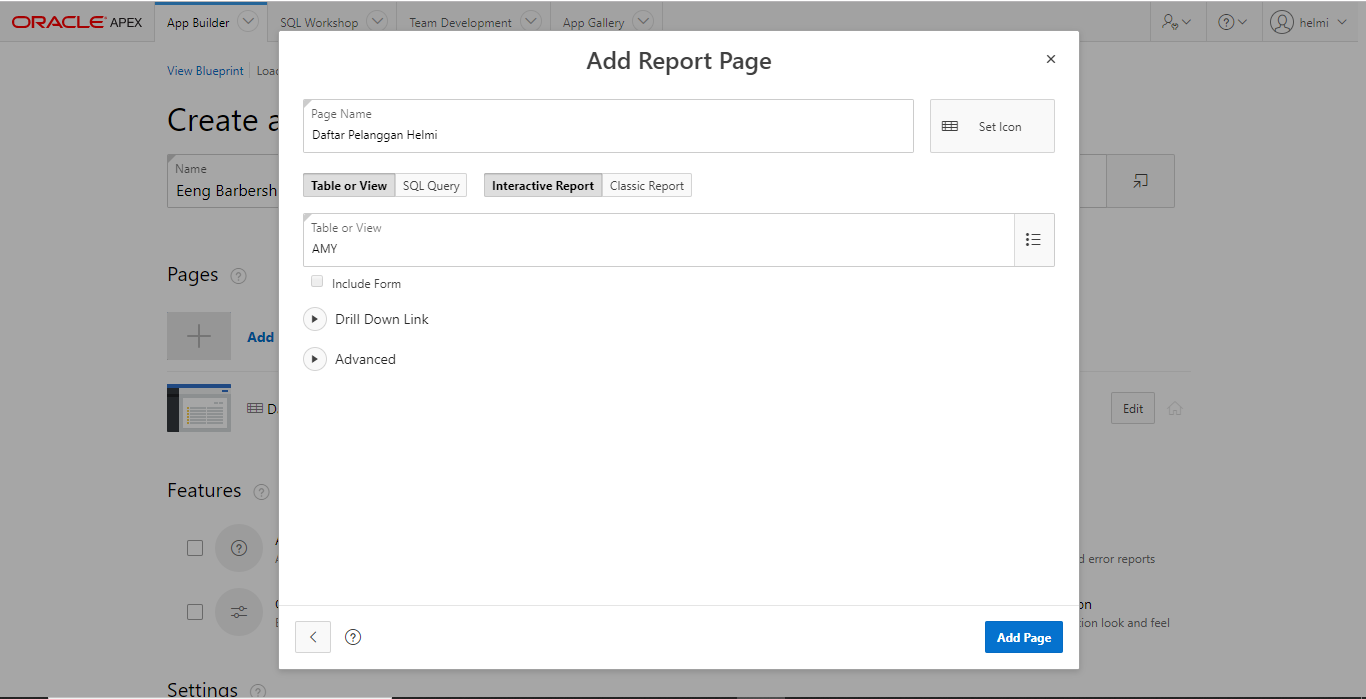
\includegraphics[scale=0.3]{gambar/12.PNG}
        \end{center}
        
         \item pilih interactive report untuk menampilkan data pelanggan yang akan dicukur oleh almi dan pilih view alm lalu page add page 
        \begin{center}
            \centering
            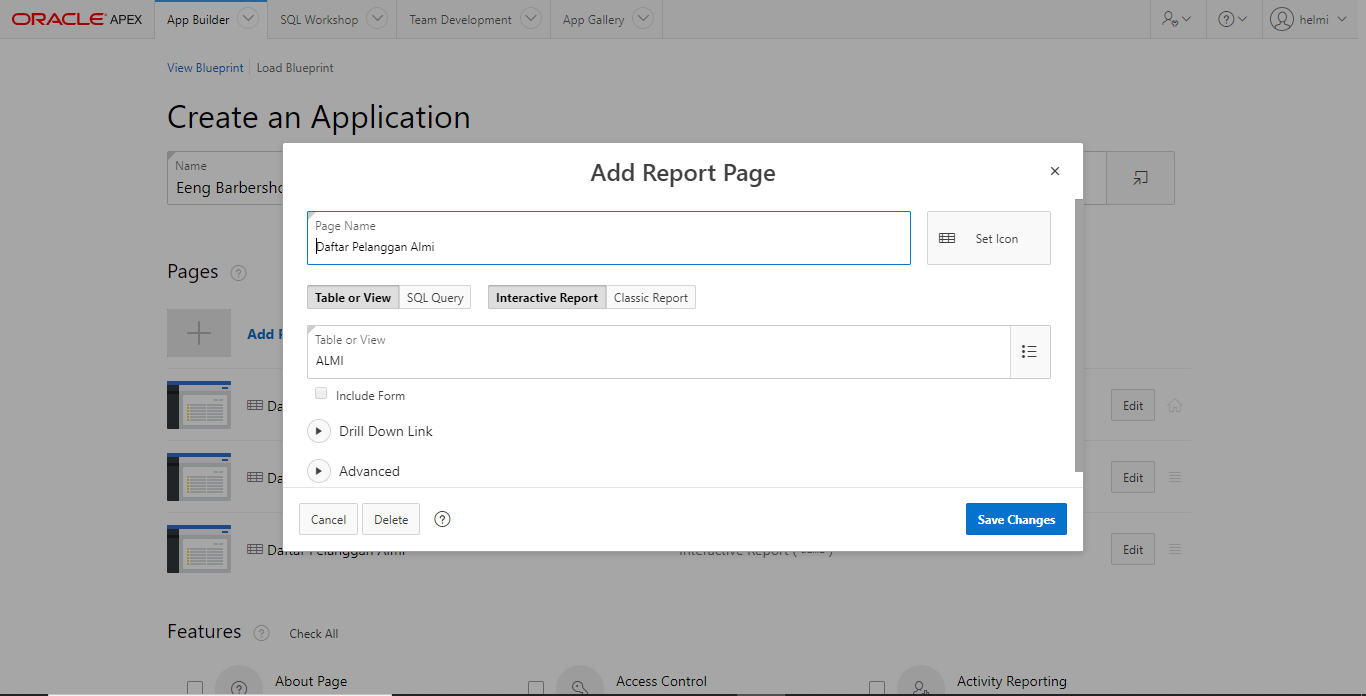
\includegraphics[scale=0.3]{gambar/13.PNG}
        \end{center}
        
        \item pilih page age lagi dan pilih form agar pelanggan dapat mendaftar 
        \begin{center}
            \centering
            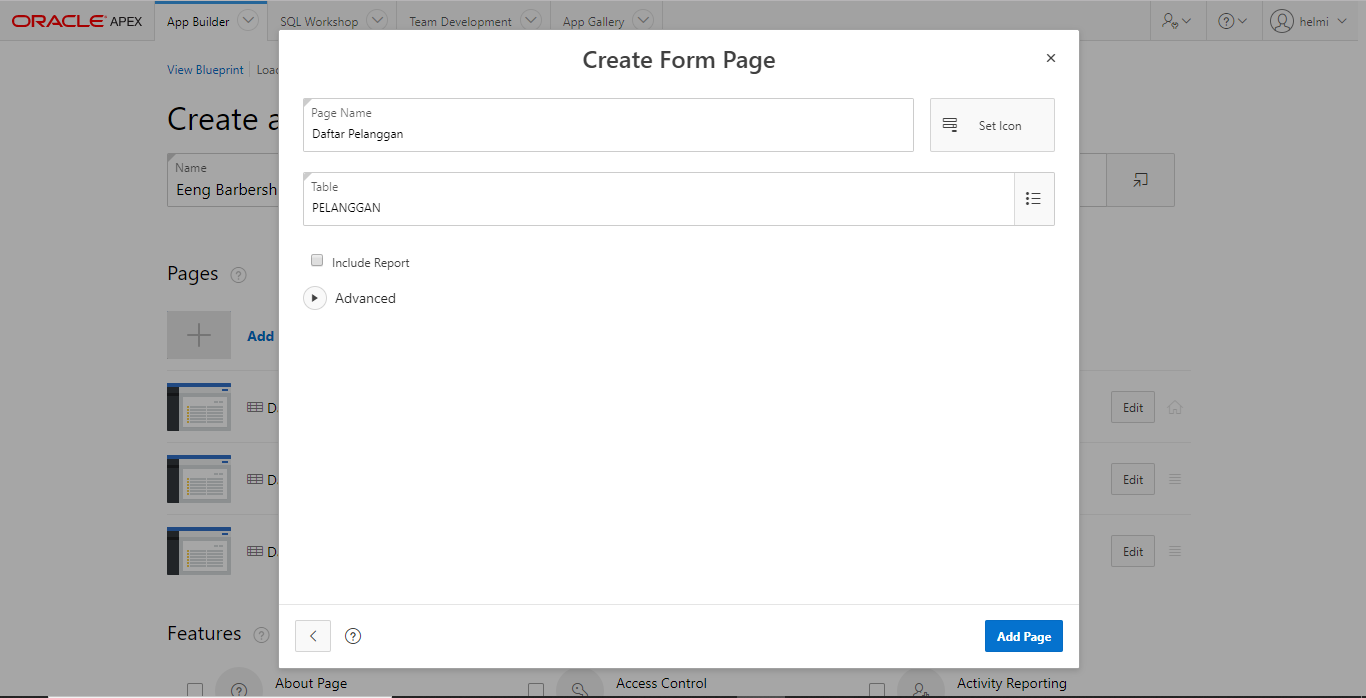
\includegraphics[scale=0.3]{gambar/14.PNG}
        \end{center}
        
        \item pilih page age lagi dan pilih master detail agar admin dapat melihat daftar barber dan pelanggan
        \begin{center}
            \centering
            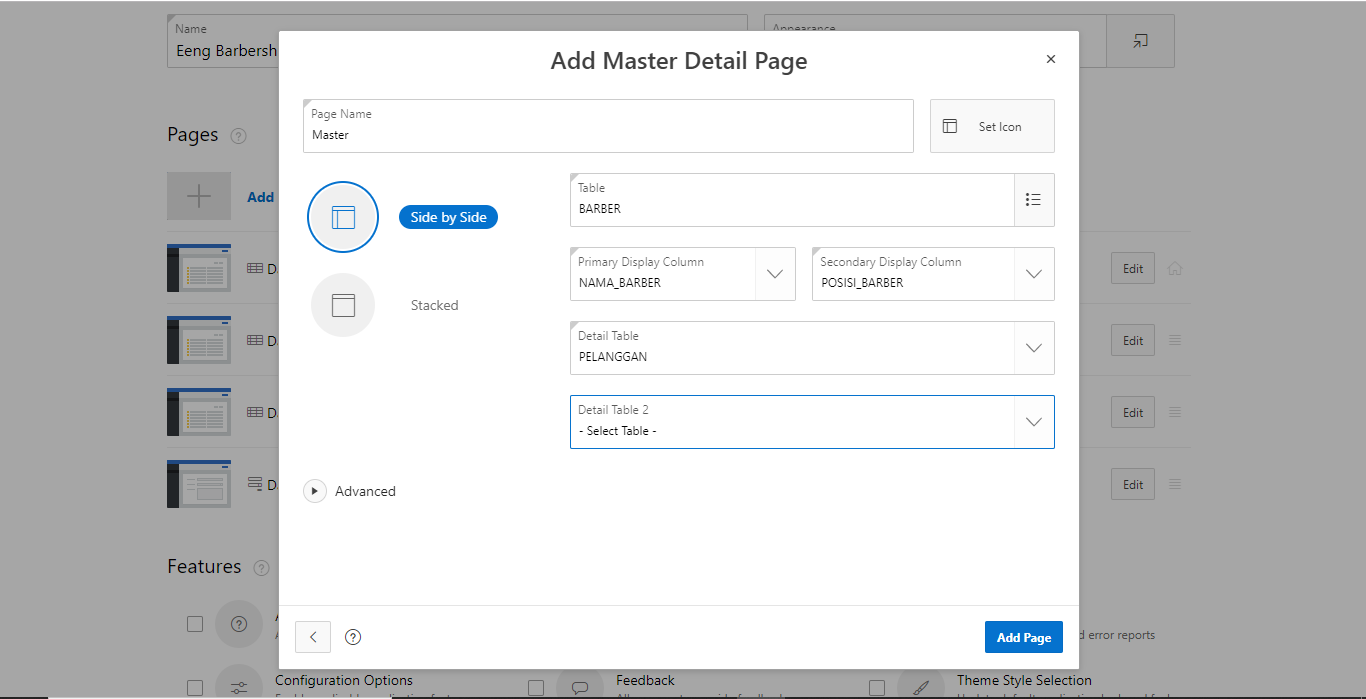
\includegraphics[scale=0.3]{gambar/15.PNG}
        \end{center}
        

        \item pilih page age lagi dan pilih interactive report dan masukan tabel history pelanggan agar dapat melihat history pelanggan
        \begin{center}
            \centering
            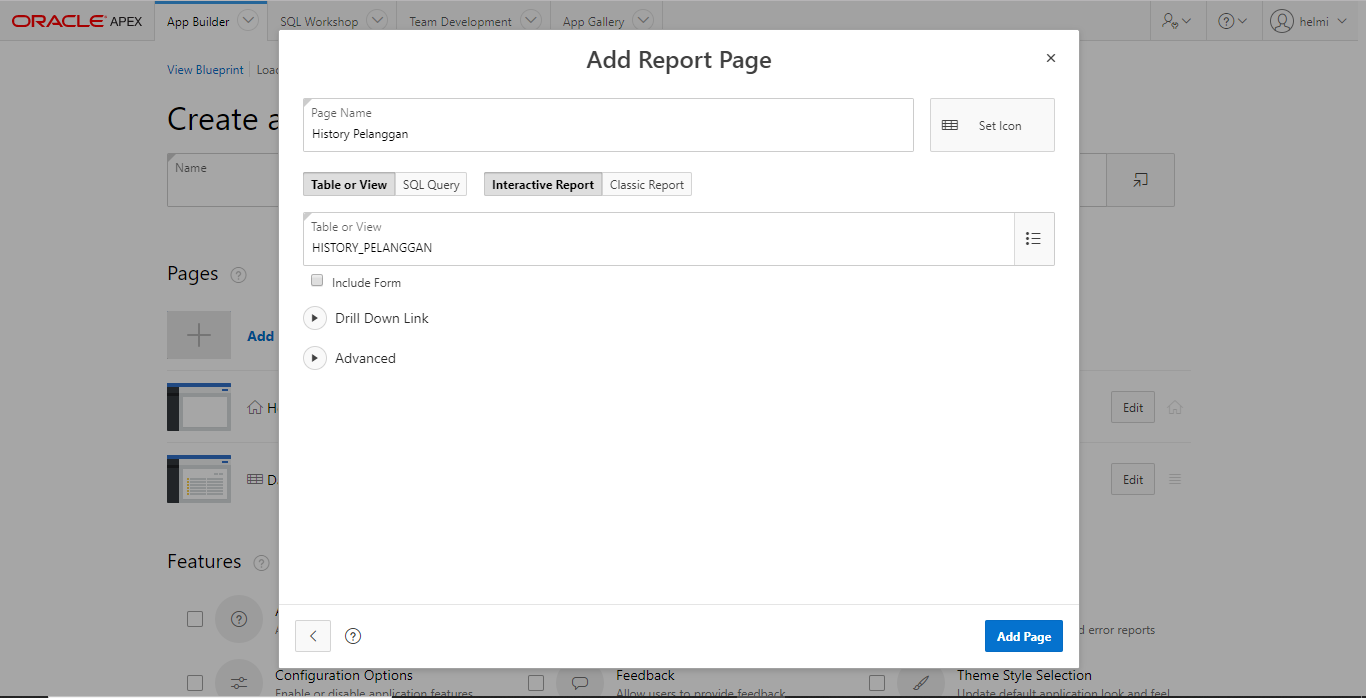
\includegraphics[scale=0.3]{gambar/22.PNG}
        \end{center}
        
        \item lalu create application
        \begin{center}
            \centering
            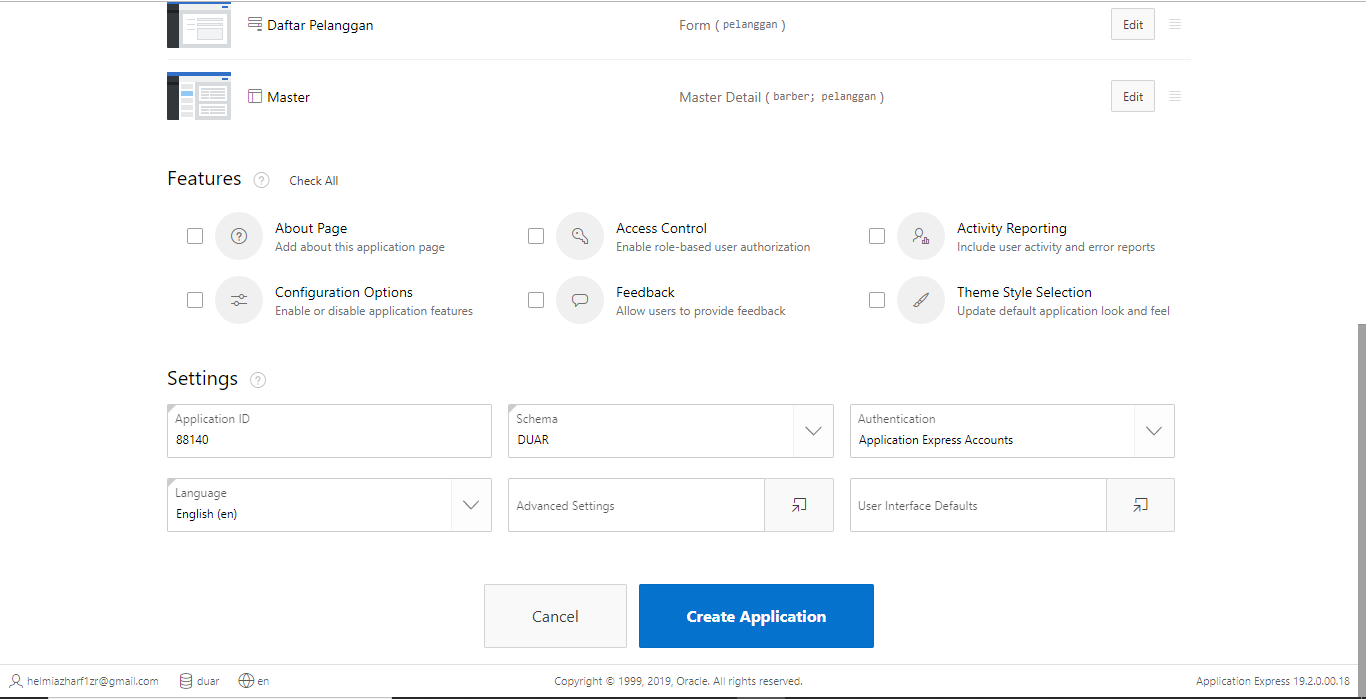
\includegraphics[scale=0.3]{gambar/16.PNG}
        \end{center}
        
        \item loading
        \begin{center}
            \centering
            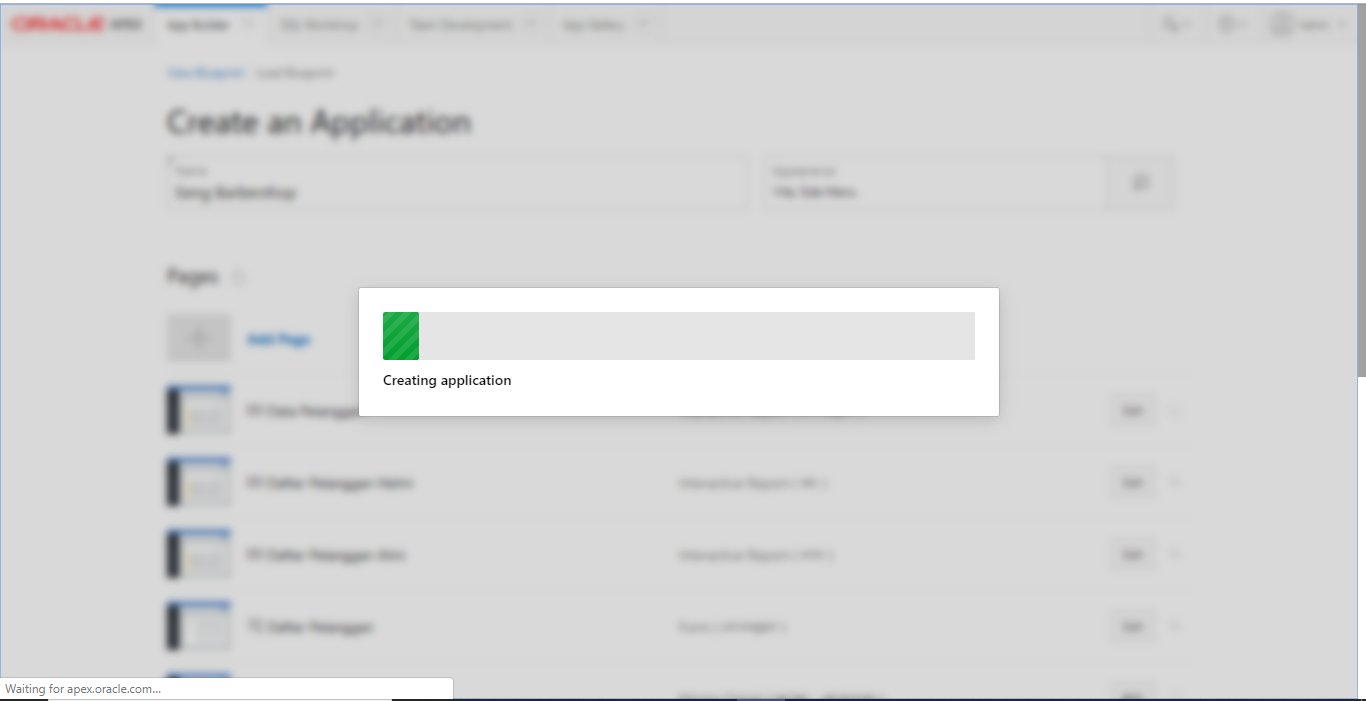
\includegraphics[scale=0.3]{gambar/17.PNG}
        \end{center}
        
         \item Setelah loading akan muncul tampilan seperti ini,lalu run application
        \begin{center}
            \centering
            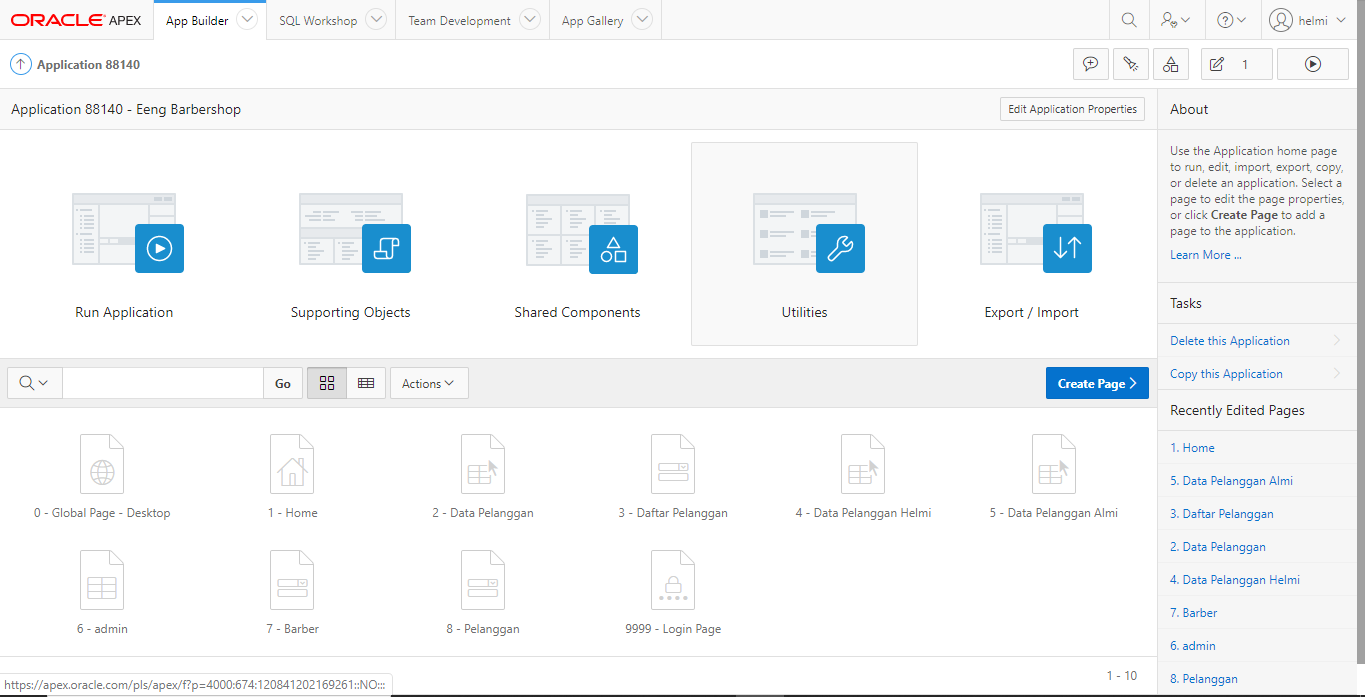
\includegraphics[scale=0.3]{gambar/19.PNG}
        \end{center}
        
        \item Masukan username dan password
        \begin{center}
            \centering
            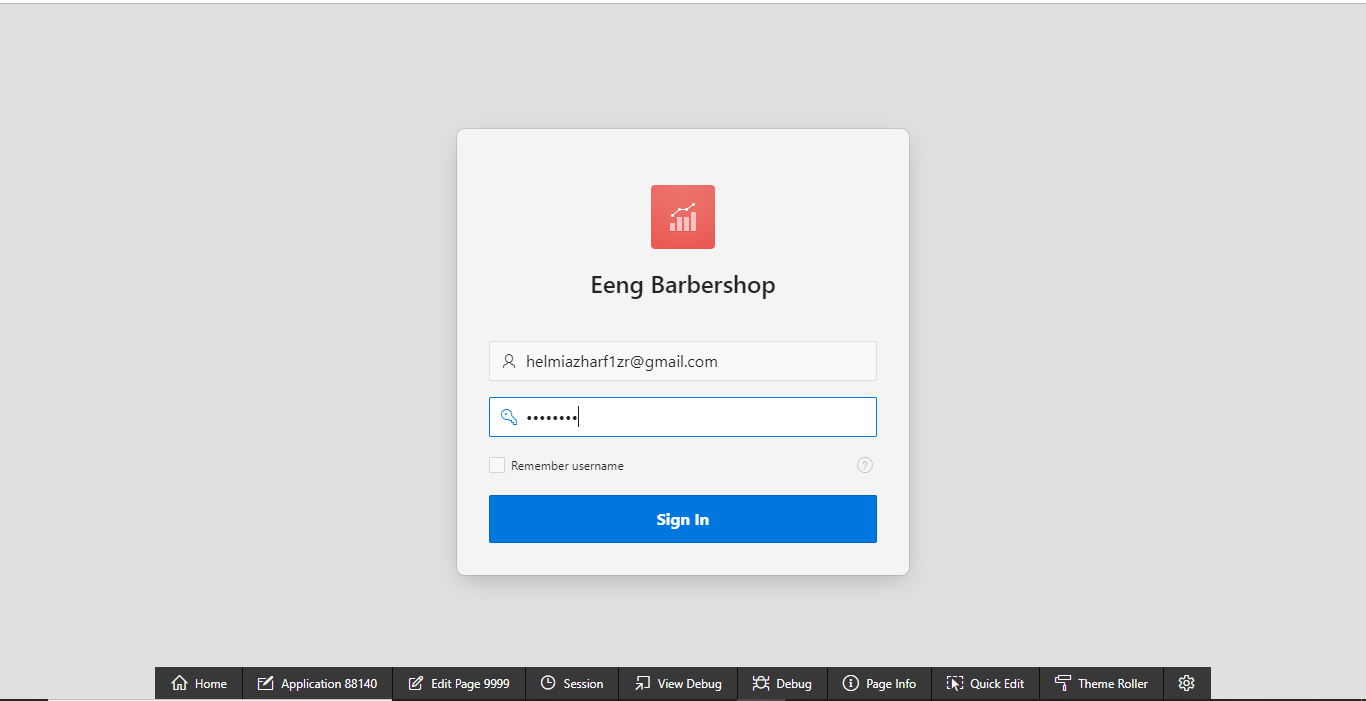
\includegraphics[scale=0.3]{gambar/20.PNG}
        \end{center}
        
        \item Aplikasi selesai
        \begin{center}
            \centering
            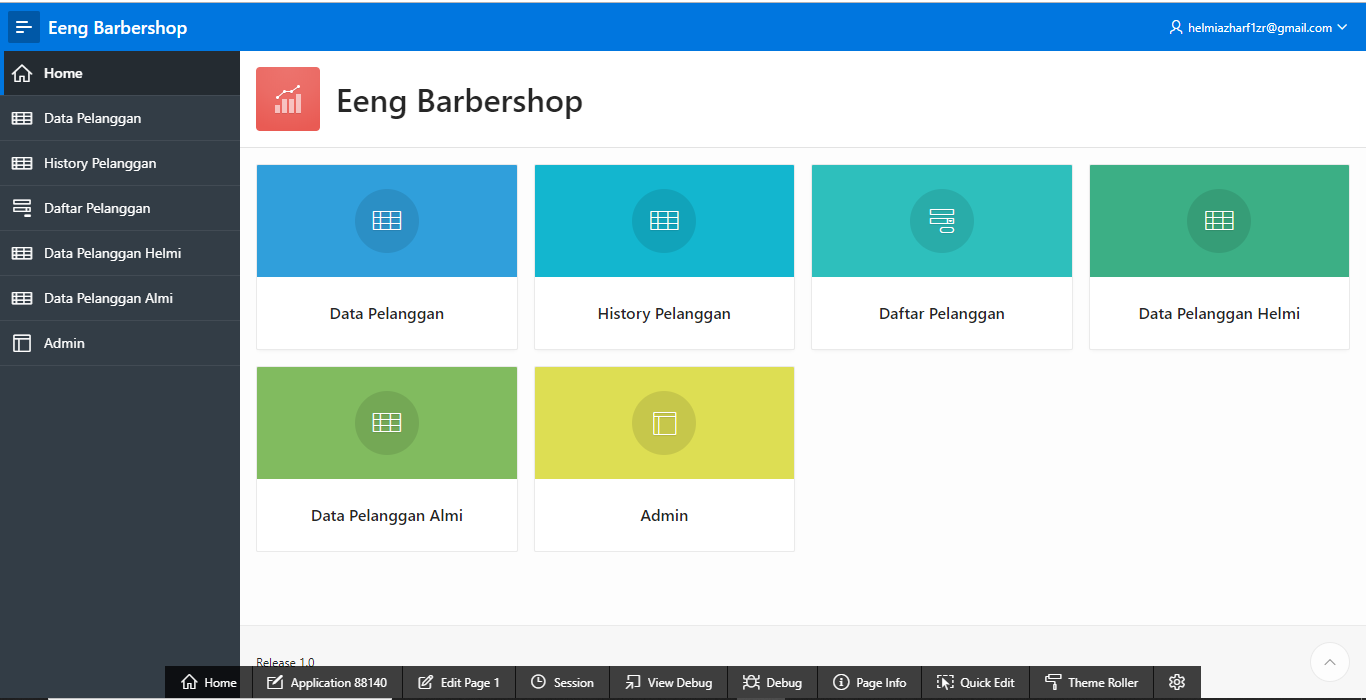
\includegraphics[scale=0.3]{gambar/21.PNG}
        \end{center}

\end{itemize}
    
\section{Data Saya}
\begin{itemize}
    \item Link      = https://apex.oracle.com/pls/apex/f?p=88140:LOGIN\textunderscore DESKTOP:1870181417415:::::
    \item Workspace = "duar"
    \item Username  = "helmiazharf1zr@gmail.com"
    \item Password  = "password"
\end{itemize}

    
\end{document}
